

\documentclass[xcolor=table]{beamer}
\usetheme{default}
\definecolor{darkscarlet}{rgb}{0.34, 0.01, 0.1}
\usecolortheme{default}
\usecolortheme[named=darkscarlet]{structure}
\setbeamercolor{title}{bg=white, fg=darkscarlet}
\definecolor{cerise}{rgb}{0.87, 0.19, 0.39}
\hypersetup{colorlinks=TRUE,linkcolor=cerise,urlcolor=cerise, citecolor=cerise}

% nummering

\setbeamertemplate{caption}[numbered]

% taal

\usepackage[english]{babel}

% tekens

\usepackage{fontspec}
\usefonttheme{serif}
\setmainfont[BoldFont=brillb.ttf, ItalicFont=brilli.ttf, BoldItalicFont=brillbi.ttf]{brill.ttf}

% tekst doorstrepen, kennelijk heb je daar een apart pakket voor nodig

\usepackage[normalem]{ulem}

% plaatjes

\usepackage{graphicx}

% tabellen

\usepackage{multirow}

% voorbeelden

\usepackage{philex}

% glossen

\usepackage{leipzig}

\newleipzig{hab}{hab}{habitual}
\newleipzig{aor}{aor}{aorist}
\makeglossaries

% bibliography

\usepackage[backend=biber,babel=other,
        bibstyle=biblatex-sp-unified,
        citestyle=sp-authoryear-comp,
        doi=false,
        maxcitenames=3,
        maxbibnames=99]{biblatex}
\addbibresource{bibliography.bib}


% custom footline

\setbeamerfont{footline}{size=\fontsize{20}{20}\selectfont}

\newcommand{\Ffootline}{\footnotesize
\insertsection
\hfill
\href{https://github.com/sverhees/}{link to Github}
\hfill
\insertframenumber/\inserttotalframenumber} 

% custom footline deel 2

\setbeamertemplate{footline}{%
\usebeamerfont{structure}
\begin{beamercolorbox}[wd=\paperwidth,ht=2.25ex,dp=1ex]{title in head/foot}%
\Tiny\hspace*{4mm} \Ffootline \hspace{4mm}
\end{beamercolorbox}}

% navigatiesymbolen uitzetten

\beamertemplatenavigationsymbolsempty
 
 
% titelpagina 

\title{Variation in two dictionaries of Botlikh}
\author{George Moroz, Chiara Naccarato, Samira Verhees \\
Linguistic Convergence Laboratory at NRU HSE Moscow}
\date{Документирование языков и диалектов коренных малочисленных народов России\\ 14--16.10.2019 - St.Petersburg}


% links

\usepackage{hyperref}

%\newcommand\pro{\item[$+$]}
%\newcommand\con{\item[$-$]} 

\begin{document}

\begin{frame}
\titlepage

\end{frame}

\section{Botlikh}
\begin{frame}{Botlikh}
\begin{itemize}
    \item Botlikh < Andic group < East Caucasian language family
    \item Unwritten (can be written with extended Cyrillic script for Avar)
    \item \textasciitilde{}5000-8000 speakers
    \item Mostly spoken in 3 villages in northwestern Daghestan (Russian Federation): Botlikh, Miarso, Ashino, (Ankho); minor dialectal differences
    \item Opinions vary on the language's vitality --- it is still passed on to children and spoken at home, but some families are shifting to Russian
    \pause
    \item One full reference grammar in Georgian  \citep{gudava1962}
    \item Two dictionaries: \\
    \citep{saidovaabusov2012} and \citep{alekseev2019}
\end{itemize}
\end{frame}

\begin{frame}{Botlikh}
\begin{figure}[h]
\centering
\fbox{\includegraphics[scale=0.4]{images/globalmap.png}}
\end{figure}
\end{frame}

\section{Data}
\begin{frame}{Two dictionaries}

\begin{block}{\citep{saidovaabusov2012}}
    \begin{itemize}
        \item Compiled in the 2000s by a native speaker (M.G. Abusov) and an experienced linguist (P.A. Saidova)
        \item Mostly Botlikh with some notes on Miarso
    \end{itemize}
\end{block}

\pause

\begin{block}{\citep{alekseev2019}}
    \begin{itemize}
        \item Compiled in the 1960s / 1970s by a native speaker / philologist (X.G. Azaev) and later (in the 2000s) systematized by an experienced linguist (M.E. Alekseev)
        \item Subsequently edited by T.A. Maisak and scheduled for posthumous publication later this year
        \item Botlikh only % проверить Алексеева, возможно туда влезали миарсинские слова
    \end{itemize}
\end{block}
\end{frame}

\begin{frame}{Two dictionaries}

\begin{itemize}
    \item Dictionaries were compiled \textit{independently} of each other
    \item \textasciitilde{}8,000 headwords \citep{saidovaabusov2012} vs. \textasciitilde{}9,000 `words and expressions' \citep{alekseev2019} % посмотреть сколько входов мы вычислили
    \item No metadata on the speakers consulted
    \item Data from \citep{alekseev2019} was collected several decades earlier, but M.G. Abusov also consulted elderly speakers with the aim of collecting archaic vocabulary (p.c.)
    \pause
    \item At first glance, the two resources seemed to display variation
\end{itemize}

\end{frame}

\begin{frame}{Two dictionaries}

\begin{center}
    \textbf{Aim of the present investigation}\\
    Compare the two resources, see to what extent they overlap and diverge, and verify whether they display systematic variation\\
    ...
    \pause
    \vfill
    and \textit{hopefully}, explain the kind of variation we found\\ (idiolectal, diachronic, etc.) 
    
\end{center}

\end{frame}

\begin{frame}{Data}
Merge dictionaries (doc to xls table) through a painstaking process of unification (\href{https://github.com/agricolamz/}{George Moroz}).

\begin{figure}[h]
\centering
\fbox{\includegraphics[scale=0.17]{images/dicts.jpg}}
\end{figure}
\end{frame}

\begin{frame}{Data}

Nouns (genitive, plural) and verbs (habitual and aorist)

\begin{figure}[h]
\centering
\fbox{\includegraphics[scale=0.4]{images/table.jpg}}
\end{figure}

\pause
From \textasciitilde{}15,000-17,000 lexical entries, we automatically extracted 7,583 nouns and verbs, further manual correction

\end{frame}


\begin{frame}{Parameters}
\begin{itemize}
    \item Phonology: word similarity, stress patterns
    \item Nominal morphology: formation of genitive case and plural forms
    \item Verbal morphology: formation of basic tenses
\end{itemize}
\end{frame}

\section{Variation}

\begin{frame}{Phonology}
For phonological analysis we used only those words which were found in both dictionaries (1,688).
\begin{itemize}
\item 1,309 words are the same
\item 254 words have difference in stress: \textit{ansːí} `warm up' (A\&A) vs. \textit{ánsːi} (S\&A)
\item and only 125 words have some segmental differences
\begin{itemize}
\item Some differences could be typos (\textit{kalχoznik'} `kolkhoz member' (A\&A) vs. \textit{kalχoznik} (S\&A), \textit{lah} (лагь) `slave' (A\&A) 2006 vs. \textit{laʁ} (лагъ) (S\&A))
\item Multiple cases where there is a small difference that could be explained either as a typo or in terms phonological variation (\textit{čuhí} `to run' (A\&A) vs. \textit{čũhí} (S\&A), \textit{kusu} `cherry plum' (A\&A) vs. \textit{kusːu} (S\&A))
\item Multiple cases where Russian borrowings were adopted differently (\textit{pojiz} `train' (A\&A) vs. \textit{poezd} (S\&A), \textit{biton} `milk can' (A\&A) vs. \textit{bitun} (S\&A))
\end{itemize}
\end{itemize}
\end{frame}


\begin{frame}{Nominal morphology}
Formation of the plural
\begin{itemize}
    \item A suffix is attached to the absolutive stem: \textit{na} `thing' < \textit{na-\textbf{baɬi}} `things'
    \item With stems ending in a consonant the vowel \textit{-a-} is often inserted before the suffix: \textit{majmalak}  `monkey' < \textit{majmalak-\textbf{a}-\textbf{baɬi}} `monkeys'
    \item With stems ending in a vowel alternation can occur: \textit{ruš\textbf{a}}  `tree' < \textit{ruš\textbf{i}-\textbf{baɬi}} `trees', \textit{sal\textbf{u}}  `tooth' < \textit{sal\textbf{a}-\textbf{baɬi}} `teeth', \textit{buraɬ\textbf{i}}  `pitcher' < \textit{buraɬ\textbf{a}-\textbf{baɬi}} `pitchers'
    \item Among the most common suffixes are: \textit{-baɬi} (and variants, e.g. \textit{-zabaɬi}, \textit{-maɬi}, etc.), \textit{-de}, \textit{-(w)e}
    %add more suffixes
\end{itemize}
\end{frame}

\begin{frame}{Nominal morphology}
Case declension (core cases)
\begin{itemize}
    \item I type --- the stem does not change when a suffix is attached (mostly stems ending in a vowel and masdars): \textit{bab\textbf{u}} `mom' < \textit{bab\textbf{u}-\textbf{ɬi}} (genitive), \textit{masir} `measurement' < \textit{masir-\textbf{ɬi}} (genitive)  
    \item II type --- case suffixes are attached to the oblique stem of the noun (mostly stems ending in a consonant, sometimes stems ending in a vowel): \textit{askar} `army' < \textit{askar-\textbf{a}-\textbf{ɬi}} (genitive), \textit{din} `religion' < \textit{din-\textbf{i}-\textbf{ɬi}} (genitive), \textit{ima} `father' < \textit{im\textbf{u}-\textbf{ɬi}} (genitive) 
\end{itemize}
\end{frame}

\begin{frame}{Nominal morphology}
\begin{itemize}
    \item Both dictionaries report both the \textbf{genitive} and the \textbf{plural} suffix
    \item We used this information to study the productivity of such suffixes, and to see whether the two dictionaries display variation
    \pause
    \item We retrieved 2,965 nouns for A\&A, 2,952 for S\&A
    \item 1,072 pairs were present in both dictionaries and had information about inflectional forms
    \pause
    \item The genitive suffix is almost always reported in both dictionaries: for all 1,072 words in S\&A, for 1,066 words in A\&A
    \item The plural is not reported for all words: for 571 words in S\&A, for 879 words in A\&A % such cases include nouns which are not normally used in the plural (e.g. abstract nouns), demonyms (because the plural form of the demonym is usually reported as a separate entry in the dictionary), masdars (Saidova&Abusov)
\end{itemize}
\end{frame}

\begin{frame}{Nominal morphology}
\begin{figure}[h]
\caption{Variation: plural suffixes}
\centering
\includegraphics[height=5.5cm]{images/plural.png}
\end{figure}
\small (X-squared = 47.118, df = 2, p-value = 5.869e-11)
\end{frame}

\begin{frame}{Nominal morphology}
\begin{table}[]
\caption{Stem endings and genitive suffix}
\centering
\begin{tabular}{|
>{\columncolor[HTML]{EFEFEF}}c |
>{\columncolor[HTML]{FFFFFF}}c |
>{\columncolor[HTML]{FFFFFF}}c |
>{\columncolor[HTML]{FFFFFF}}c |
>{\columncolor[HTML]{FFFFFF}}c |
>{\columncolor[HTML]{FFFFFF}}c |
>{\columncolor[HTML]{FFFFFF}}c |
>{\columncolor[HTML]{FFFFFF}}c |
>{\columncolor[HTML]{FFFFFF}}c |}
\hline
\textbf{Suffix} & \multicolumn{2}{c|}{\cellcolor[HTML]{EFEFEF}\textit{-ɬi}} & \multicolumn{2}{c|}{\cellcolor[HTML]{EFEFEF}\textit{-aɬi}}                                                                & \multicolumn{2}{c|}{\cellcolor[HTML]{EFEFEF}\textit{-iɬi}}                                                                & \multicolumn{2}{c|}{\cellcolor[HTML]{EFEFEF}\textit{-uɬi}} \\ \hline
\textbf{Stem}   & {\color[HTML]{009901} S\&A} & {\color[HTML]{F56B00} A\&A} & {\color[HTML]{009901} S\&A}                                 & {\color[HTML]{F56B00} A\&A}                                 & {\color[HTML]{009901} S\&A}                                 & {\color[HTML]{F56B00} A\&A}                                 & {\color[HTML]{009901} S\&A}  & {\color[HTML]{F56B00} A\&A} \\ \hline
consonant       & {\color[HTML]{009901} 232}  & {\color[HTML]{F56B00} 266}  & \cellcolor[HTML]{ECF4FF}{\color[HTML]{009901} \textbf{228}} & \cellcolor[HTML]{ECF4FF}{\color[HTML]{F56B00} \textbf{167}} & \cellcolor[HTML]{ECF4FF}{\color[HTML]{009901} \textbf{104}} & \cellcolor[HTML]{ECF4FF}{\color[HTML]{F56B00} \textbf{141}} & {\color[HTML]{009901} -}     & {\color[HTML]{F56B00} 1}    \\ \hline
\textit{-a}     & {\color[HTML]{009901} 182}  & {\color[HTML]{F56B00} 167}  & {\color[HTML]{009901} -}                                    & {\color[HTML]{F56B00} -}                                    & \cellcolor[HTML]{ECF4FF}{\color[HTML]{009901} 3}            & \cellcolor[HTML]{ECF4FF}{\color[HTML]{F56B00} 13}           & {\color[HTML]{009901} 15}    & {\color[HTML]{F56B00} 14}   \\ \hline
\textit{-i}     & {\color[HTML]{009901} 143}  & {\color[HTML]{F56B00} 151}  & \cellcolor[HTML]{ECF4FF}{\color[HTML]{009901} 10}           & \cellcolor[HTML]{ECF4FF}{\color[HTML]{F56B00} 4}            & {\color[HTML]{009901} -}                                    & {\color[HTML]{F56B00} -}                                    & {\color[HTML]{009901} 3}     & {\color[HTML]{F56B00} 2}    \\ \hline
\textit{-u}     & {\color[HTML]{009901} 81}   & {\color[HTML]{F56B00} 78}   & {\color[HTML]{009901} 1}                                    & {\color[HTML]{F56B00} -}                                    & {\color[HTML]{009901} -}                                    & {\color[HTML]{F56B00} 3}                                    & {\color[HTML]{009901} -}     & {\color[HTML]{F56B00} -}    \\ \hline
\textit{-e}     & {\color[HTML]{009901} 6}    & {\color[HTML]{F56B00} 6}    & {\color[HTML]{009901} -}                                    & {\color[HTML]{F56B00} -}                                    & {\color[HTML]{009901} -}                                    & {\color[HTML]{F56B00} -}                                    & {\color[HTML]{009901} -}     & {\color[HTML]{F56B00} -}    \\ \hline
\textit{-o}     & {\color[HTML]{009901} 7}    & {\color[HTML]{F56B00} 7}    & {\color[HTML]{009901} -}                                    & {\color[HTML]{F56B00} -}                                    & {\color[HTML]{009901} -}                                    & {\color[HTML]{F56B00} -}                                    & {\color[HTML]{009901} -}     & {\color[HTML]{F56B00} -}    \\ \hline
\end{tabular}
\end{table}
\end{frame}

\begin{frame}{Nominal morphology}
\begin{figure}[h]
\centering
\caption{Variation: genitive in \textit{-aɬi} vs. \textit{-iɬi} with stems ending in a consonant}
\includegraphics[height=5.5cm]{images/genitive.png}
\end{figure}
\small (X-squared = 13.523, df = 1, p-value = 0.0002357)  
\end{frame}

\begin{frame}{Nominal morphology}
\begin{center}Variation: examples
\end{center}
\begin{itemize}
    \item It seems that variation frequently involves loanwords: 
    \begin{itemize}
        \item \textit{dakument} `document' < \textit{dakument-\textbf{aɬi}} (genitive, S\&A) vs. \textit{dakument-\textbf{iɬi}} (genitive, A\&A)
        \item \textit{birgadir} `foreman' < \textit{birgadir-\textbf{zabaɬi}} (plural, S\&A) vs. \textit{birgadir-\textbf{de}} (plural, A\&A)
        \item \textit{kassir} `cashier' < \textit{kassir-\textbf{aɬi}} (genitive, S\&A), \textit{kassir-\textbf{zabaɬi}} (plural, S\&A) vs. \textit{kassir-\textbf{iɬi}} (genitive, A\&A), \textit{kassir-\textbf{de}} (plural, A\&A)
    \end{itemize}
    \pause
    \item But not only:
    \begin{itemize}
        \item \textit{gač'a} `hoe' < \textit{gač'a-\textbf{ɬi}} (genitive, S\&A), \textit{gač'-\textbf{ibaɬi}} (plural, S\&A) vs. \textit{gač'-\textbf{iɬi}} (genitive, A\&A), \textit{gač'-\textbf{e}} (plural, A\&A)
    \end{itemize}
\end{itemize}
\end{frame}

\begin{frame}{Verbal morphology}

\begin{itemize}
    \item We retrieved 1,570 verbal entries for A\&A and 1,475 for S\&A 
    \item Only 554 pairs were present in both dictionaries and had information about inflectional forms
    \pause
    \item Botlikh has only one verb stem; suffixes are attached directly
    \item Infinitive and Aorist are indicative for conjugation:
    \pause

\begin{table}[h]
\caption{Basic verb inflection in Botlikh}
\label{tab:verbtense}
\begin{tabular}{l|l|l|l}
          & \multicolumn{1}{c|}{infinitive} & \multicolumn{1}{c|}{present} & \multicolumn{1}{c}{past} \\ \hline
Basic     & -i                              & -e                           & -a / -u / -iw            \\
Derived   & -ɬi                             & b-ah-e                       & b-ah-u `become'          \\
          &                                 & b-uk'-e                      & b-uk'-a `be'             \\
Causative & -a-j                            & mal-e / malih-e              & -o / malih-u            
\end{tabular}
\end{table}
\end{itemize}

\end{frame}

\begin{frame}{Verbal morphology}

\begin{figure}[h]
\centering
\caption{Past tense suffixes in the sample of common verbs}
\includegraphics[scale=0.5]{images/pst.png}
\end{figure}
\end{frame}

\begin{frame}{Verbal morphology}

\begin{itemize}
    \item There is more variation than the plot shows

\begin{table}[]
\caption{Past suffixes in both dictionaries}
\label{tab:pstcorr}
\begin{tabular}{l|cccc}
S\&A / A\&A & \multicolumn{1}{l}{a} & \multicolumn{1}{l}{iw} & \multicolumn{1}{l}{u} & \multicolumn{1}{l}{other} \\ \hline
a           & 72                    & 6                      & 3                     & 4                         \\
iw          & 3                     & 55                     & 6                     & 3                         \\
u           & 3                     & 4                      & 142                   & 2                         \\
other       & 3                     & 1                      & 4                     & 0                        
\end{tabular}
\end{table}
\pause
\vfill
\item But still not a lot
\item And no systematic correspondence
\end{itemize}
\end{frame}

\begin{frame}{Verbal morphology}

\begin{figure}[h]
\centering
\caption{Past tenses in all dictionary data}
\includegraphics[scale=0.4]{images/pstfull.png}
\end{figure}

\small (x-squared = 0.347, df = 2, p-value = 0.8407) %p-value > 0.05, we cannot reject the 0 hypothesis that the dictionaries are the same

\end{frame}


\begin{frame}{Verbal morphology}

\begin{figure}[h]
\centering
\caption{Infinitive vs. past tense}
\includegraphics[scale=0.45]{images/infxpst.png}
\end{figure}

\end{frame}


\begin{frame}{Verbal morphology}

\begin{table}[h]
\caption{Causative paradigms in Botlikh}
\label{tab:caus}
\begin{tabular}{l|l|l|l}
     & \multicolumn{1}{c|}{infinitive} & \multicolumn{1}{c|}{present} & \multicolumn{1}{c}{past} \\ \hline
A\&A & -a-j                            & malih-e                      & malih-u                  \\
     &                                 & -e                           & -o                       \\ \hline
S\&A & -a-j                            & mal-e                        & -o                       \\
     &                                 & -e                           & -o                       \\
     &                                 & mal-e                        & mal-o (1x)                  
\end{tabular}
\end{table}

\pause

\begin{itemize}
    \item The bulk of material in A\&A was collected several decades earlier with respect to S\&A
    \item It seems that in contemporary Botlikh, the present form \textit{malih-e} has been reduced to \textit{mal-e} and the past form \textit{malih-u} has been replaced by \textit{-o}, formerly reconstructed as \textless \textit{*-a-u} [\textsc{-caus-pst}]
\end{itemize}
\end{frame}


\begin{frame}{Verbal morphology}

\begin{figure}[h]
\centering
\caption{Infinitive vs. present tense}
\includegraphics[scale=0.45]{images/infxprs.png}
\end{figure}

\end{frame}

\begin{frame}{Verbal morphology}

Correspondence between infinitive and present tense form

\begin{itemize}
    \item Illustrates the division in causative forms (cf. Table \ref{tab:caus}): full form \textit{malihe} in A\&A, shorter form \textit{male} in S\&A
    \pause
    \item Preference for a specific auxiliary to inflect derived verbs: \textit{b-ahe} `become' in A\&A, \textit{b-uk'a} `be' in S\&A
    \item This is also the case in the past
\end{itemize}
\end{frame}

\begin{frame}{Verbal morphology}

\textsc{Entry `bleat'} \textbf{baʕada/ɬí}, \textit{prs.} \textbf{bahé}, \textit{pst.} \textbf{báhu} \citep{alekseev2019}

\lb{ex:lamb}{\gll ha-b ƛ'et'ír \textbf{baʕáda} \textbf{b-uk'-é}\\
{\Dem}-{\N} lamb bleat {\N}-be-{\Hab}\\
\trans `That lamb often bleats.'}

\pause
\vfill

\textsc{Entry `roar'} \textbf{buːda/ɬí}, \textit{prs.} \textbf{buké}, \textit{pst.} \textbf{búk'a} \citep{saidovaabusov2012}

\lb{ex:ox}{\gll únsa \textbf{buːda} \textbf{b-áh-u}\\
ox roar {\N}-become-{\Aor}\\
\trans `The ox started to roar.'}
\end{frame}

\section{Summary}

\begin{frame}{Summary}
\begin{itemize}
    \item Little phonological variation besides different stress patterns in 254 words from a 1,688 word sample
    \item Nouns show some variation both in the genitive and in the plural
    \begin{itemize}
        \item A general preference for \textit{-baɬi} over \textit{-de} in the plural and for \textit{-aɬi} over \textit{-iɬi} in the genitive in S\&A
        \item The opposite trends in A\&A
        \item Variation frequently involves loanwords
        \item In some cases the dictionaries report more than one variant for both the genitive and the plural, so we might conclude that idiosyncratic variation is at play
        \pause
        \item But more research is needed!
    \end{itemize}
\end{itemize}
\end{frame}

\begin{frame}{Summary}
\begin{itemize}
    \item Verbs show diachronic and idiosyncratic variation
    \begin{itemize}
        \item The auxiliary used to derive the present tense of causatives has undergone morphologization: \textit{malihe} --- \textit{male}
        \item Some causatives (can) have a regular suffix \textit{-e}
        \item The past tense of the causative is formed with a suffix \textit{-o}, which replaced an auxiliary \textit{malihu}
        \item It remains unclear how \textit{-o} emerged
        \end{itemize}
    \end{itemize}
\end{frame}

\begin{frame}{Summary}
    \begin{itemize}
    \item Verbs show diachronic and idiosyncratic variation
        \begin{itemize}
        \item Each dictionary prefers a different auxiliary as citation form for the inflection of \textit{-ɬi} forms (derived verbs): `become' in A\&A, `be' in S\&A
        \item This is a matter of personal taste: examples in the entries of these verbs show that both are possible
        \item It seems the auxiliaries form a kind of aspectual opposition: inchoative (`become') vs. durative (`be') %but we have to check whether all verbs can take either auxiliary
        \pause
        \item Limited variation in other parts of the verbal domain
        \end{itemize}
    \end{itemize}
\end{frame}

\section{The end}
\begin{frame}{Спасибо}
\begin{figure}[h]
\centering
\fbox{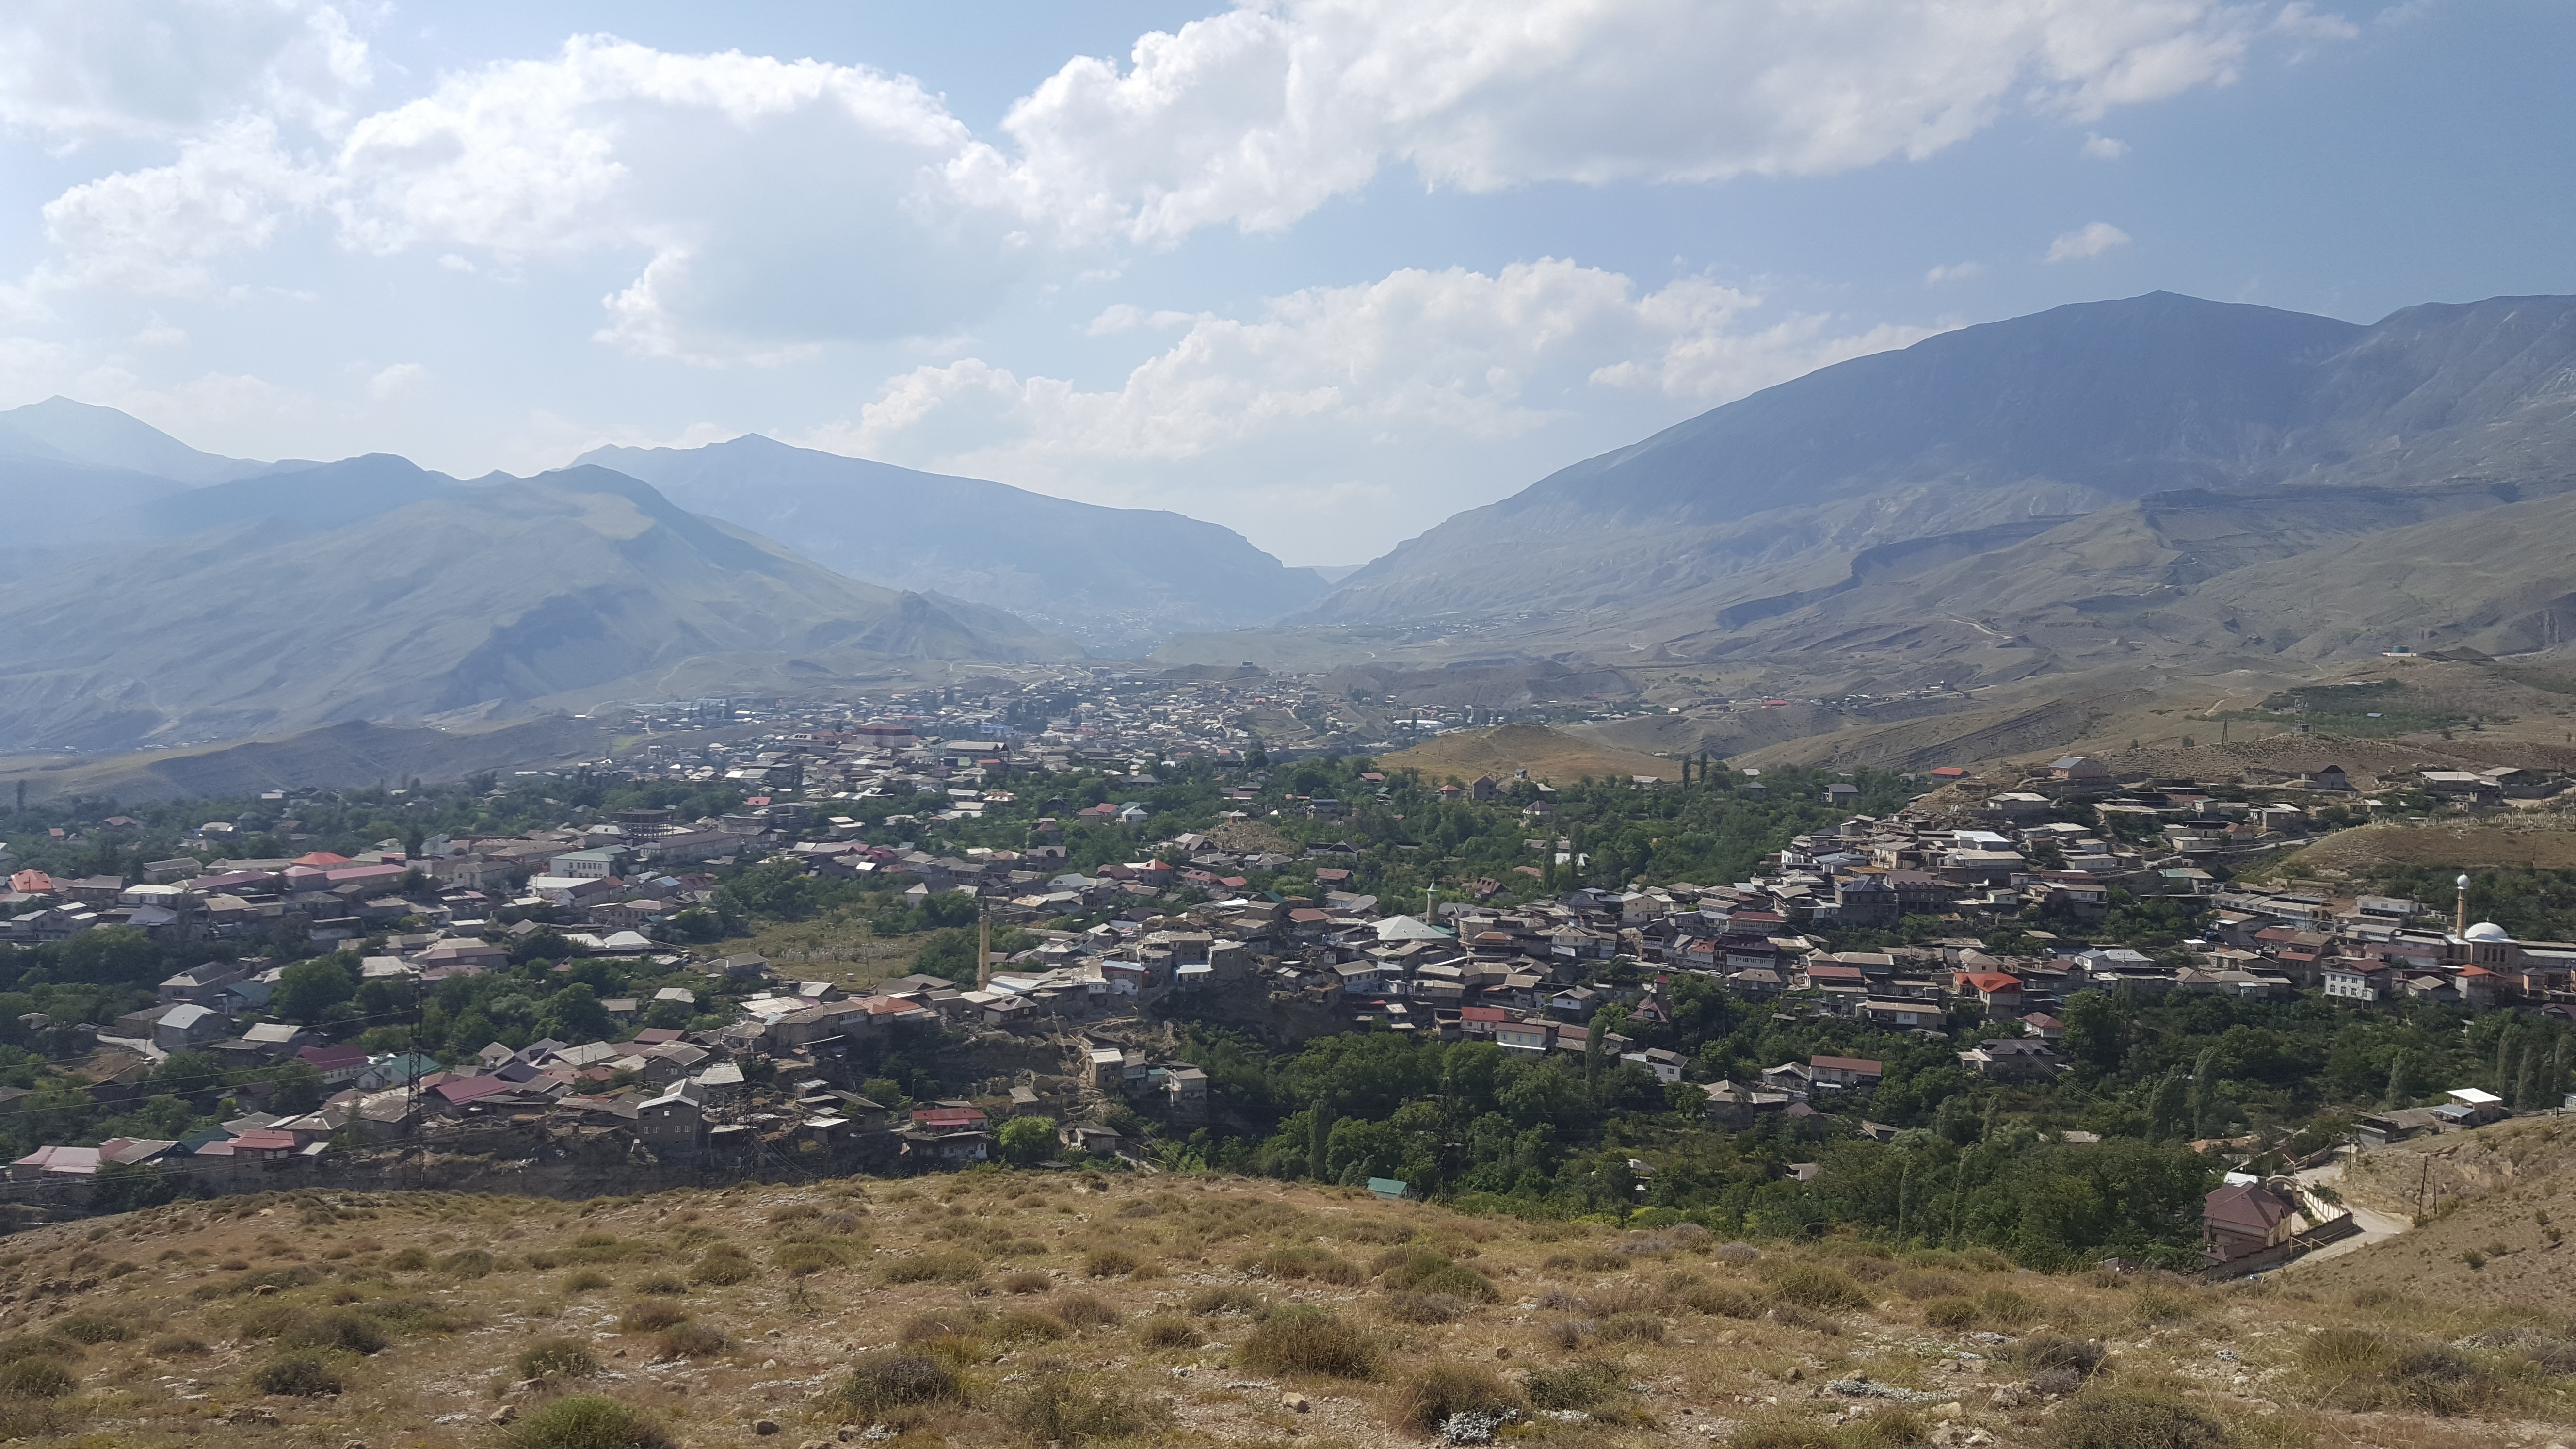
\includegraphics[height=6cm]{images/panorama.jpg}}
\end{figure}
\end{frame}

\section{Abbreviations}
\begin{frame}{Abbreviations}

\tiny{\printglossary}

\end{frame}

\section{References}
\begin{frame}{References}

\printbibliography

\end{frame}

\end{document}